\documentclass[UTF8]{ctexart}
\usepackage{titlesec}
\usepackage{listings}
\usepackage{xcolor}
\usepackage{graphicx}
\usepackage{geometry}
\usepackage{fancyhdr}
\usepackage[colorlinks, linkcolor=black]{hyperref}
\geometry{left = 2.5cm, right = 2.5cm, top = 2.0cm, bottom = 2.0cm}
\pagestyle{fancy}
\lhead{上海交通大学}
\chead{}
\rhead{电子信息及电气工程学院}
\lfoot{}
\cfoot{\thepage}
\rfoot{}
\definecolor{CPPLight}  {HTML} {686868}
\definecolor{CPPSteel}  {HTML} {888888}
\definecolor{CPPDark}   {HTML} {262626}
\definecolor{CPPBlue}   {HTML} {4172A3}
\definecolor{CPPGreen}  {HTML} {487818}
\definecolor{CPPBrown}  {HTML} {A07040}
\definecolor{CPPRed}    {HTML} {AD4D3A}
\definecolor{CPPViolet} {HTML} {7040A0}
\definecolor{CPPGray}  {HTML} {B8B8B8}
\title{手写数字识别}
\author{\\* 林伟鸿\\* \\*上海交通大学\\*\\*电子信息及电气工程学院\\*\\*计算机科学与技术\\*\\*}
\date{2016-9-21}
\begin{document}
\maketitle
\newpage
\tableofcontents

\newpage
\section{问题简述}
这里的手写数字识别是指将手写的单个数字变为统一规格的图片格式,并用计算机程序对图片进行处理,最后达到让计算机能够识别手写数字的目的。\\ \par
\centerline{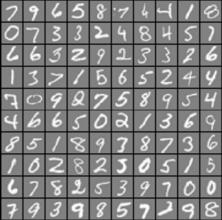
\includegraphics[height=6cm,width=6cm]{p1.jpg}}
\begin{center} 图一 \end{center}\par
如图一所示,本次我让机器识别的对象就是这种样子的图片,我对图片进行了统一处理,每张图都变成一个28*28的矩阵,每个位置代表图片该处的灰暗度。数据来源是
\url{http://yann.lecun.com/exdb/mnist/}。上面可以下载到$60000$个带有标记的训练数据以及$10000$个带有标记的测试数据。\par
手写数字识别作为机器学习的一个入门性的问题,我采用结构最简单的$BP$神经网络来处理这些图片。

\newpage
\section{$BP$神经网络}
    \subsection{简介}
$BP$($Back Propagation$)神经网络是$1986$年由$Rumelhart$和$McCelland$为首的科学家小组提出,是一种按误差逆传播算法训练的多层前馈网络,是目前应用最广泛的神经网络模型之一。$BP$网络能学习和存贮大量的输入$-$输出模式映射关系,而无需事前揭示描述这种映射关系的数学方程。它的学习规则是使用梯度下降法,通过反向传播来不断调整网络的权值和阈值,使网络的误差平方和最小。$BP$神经网络模型拓扑结构包括输入层($input$)、隐含层($hidden layer$)和输出层($output layer$)。可以证明,三层$BP$神经网络可以拟合出所有非线性函数,也就是理论上可以完成全部$n$维到$m$维的映射,因此我们下面来讨论三层的$BP$神经网络。
    \subsection{算法介绍}
我们都知道人类大脑内部有很多互相联系的神经元,它们互相连接并且传递信息,通过神经网内大量神经元的相互刺激,人类能学会各种各样复杂的事物,而神经网络算法就是以此为借鉴提出的一种让机器去学习某些事物并学会分类或者判断某些性质的算法。\\ \par
\centerline{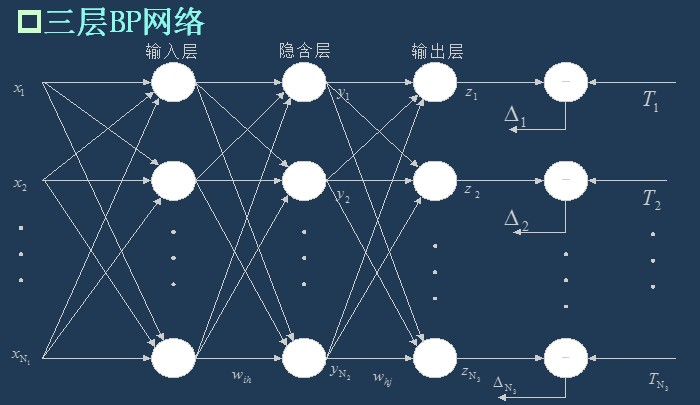
\includegraphics[height=6cm,width=12cm]{p2.jpg}}
\begin{center} 图二 \end{center}\par
如图二所示,这就是$BP$神经网络的大体结构图。该网络分为三层,分别是输入层、隐含层以及输出层。\par
        \subsubsection{输入层}
输入层一般是向网络输入一个多维的向量$\{x1,x2,...,xn\}$,该向量可以是训练的数据(用于调整网络参数)也可以是测试的数据(用于网络做出判断)。在我们研究的这个问题中,输入向量为$28*28=784$维的向量,每一维代表其灰暗度。为了提高最终识别的正确率,经过观察,我发现如果比较灰暗的地方设为$1$、而比较浅的地方设为$0$,也就是将图片变成$28*28$的$01$矩阵从肉眼的角度来说更容易辨认。因此我将这些向量进行归一化处理,全部变成非$0$即$1$的多维向量用于输入神经网络。\par
        \subsubsection{隐含层}
隐含层有一些神经节点,这些节点会从输入层接受信息,经过计算得出该节点的权值,然后通过连接的边把这一权值传送到输出节点去。隐含层的节点数是自己设定的,不同的节点所带来的效果也不一样,并非越多越好(这里主要考虑训练效率以及最终使用的正确率)。神经元权值计算公式如下:
$$W_i = \sum _{j=1} ^n (w_{ij}x_j) - \lambda_i$$ \par
上式中,$W_i$代表第$i$个节点的权值,输入向量一共$n$维,$w_{ij}$代表输入向量第$j$维与第$i$ 个神经元之间连边的权值,$\lambda_i$表示每个神经元各自的偏置值,我们可以认为,对于同样的信息同样的来源,不同的神经元可能也会有自己不同的理解。计算完隐含层每个神经元的权值,我们再利用一个激活函数$f(x)$,将其映射到一个固定值域上。
$$y_i = f(x_i)$$ \par
对于我们研究的这个问题,我所采用的激活函数为:
$$f(x) = \frac{1}{1 + e^{-x}}$$ \par
这个函数的值域为$[0,1]$,并且求导起来也方便,这点后面会用到。\par
        \subsubsection{输出层}
输出层接收隐含层神经节点传输来的数据,并采用同样的方法映射成一个值域上的数值,然后程序就可以根据输出层的各个节点权值做出判断了。在我们研究的问题中,因为单个数字一共有$10$种可能,所以我们设置了$10$个输出节点,每个节点最后得到一个$[0,1]$的权值。\par
输出层节点权值计算公式:
$$W_k = \sum _{i=1} ^m (w_{ki}y_i) - \lambda_k$$ \par
上式中,$W_k$代表第$k$个输出神经节点的权值,$w_{ki}$代表隐含层第$i$个节点与第$k$个输出神经元之间连边的权值,$\lambda_k$表示每个输出神经元的偏置值。\par
同样地,我们利用激活函数$f(x)$将输出节点的权值映射到$[0,1]$这个区间上。最后,我们认为权值最高的输出神经点所代表的数字即为答案。\par
    \subsection{反馈与调节}
看了$BP$神经网络的工作原理,我们不难发现:网络中边与点的一些基础权值会直接决定该网络工作时的正确率。假如一开始所有基础权值都通过随机得到,要想提高网络的正确率,就要通过不断地调节这些权值以达到一个相对训练样本而言较为稳定的状态,而$BP$神经网络就具有这种反馈调节机制。\par
其实这个过程也很像人类自身的学习过程,我们看到一个新的事物,然后会得到某些关于该事物的信息,接着我们就会对这个事物具有一定的概念,而不断地接触各种各样的事物,我们就会不停地调整这些概念,已达到区分这些东西的目的。\par
$BP$神经网络的反馈调节过程大致可以分为三步:
\begin{enumerate}
\item[·]将训练样本数据输入神经网络,并得到各个节点的权值数据。
\item[·]根据输出节点的权值数据以及该训练样本标记所代表的期望数据作对比,得出误差参数。
\item[·]根据误差参数调整网络中的各个基础权值,使其更接近于期望。
\end{enumerate} \par
接下来我们来讲一讲如何调节参数。\par
首先,我们先定义一个期望值,我们考虑一个训练样本数据,那么其有一个标记,也就是这张图的答案。之前我们提到过,我们最终会从$10$个输出节点中取权值最高的节点所代表的数字作为答案,再加上我们选用的激活函数$f(x)$的值域为$[0,1]$,所以我们不妨定义期望结果为$\{0,0,...,1,...,0\}$,即如果答案数字为$x$,那么$x$所代表的输出节点权值为$1$,其余输出节点都为$0$,这样我们就可以根据这个期望算出误差来调节整张网络了。\par
接下来是计算误差与调整权值,我们先计算输出点的误差,调整隐含层与输出层之间边的权值以及输出层的偏置量,然后再利用输出层的误差计算出隐含层的误差,最后调整输入层与隐含层之间边的权值以及隐含层的偏置量。\par
输出层节点的误差很好算:
$$D_k = E_k - y_k$$ \par
其中,$D_k$代表第$k$个输出节点的误差,$E_k$代表该点的期望权值,$y_k$代表网络计算后得出的该点激活后的权值。\par
然后,我们就可以利用$D_k$来调节隐含层与输出层各条边的权值了。在调节的过程中,我们为了让网络的误差能够尽快收敛,采用梯度下降的方法,具体推导这里就略去了,上网搜索一下就有一大片,下面直接来看结论:
$$\Delta W_{kj} = \eta * D_k * f'(x_k) * y_j$$ \par
上式中,$W_{kj}$表示$j$号隐含层节点与$k$号输出层节点之间边权的增量,$\eta$表示是学习率,是一个一开始就定好的常数,一般为$(0,1)$区间上的一个点,$D_k$表示$k$号输出节点的误差,$f'(x_k)$ 表示$f(x_k)$ 的导数,$x_k$ 为$k$号输出节点激活前的权值,$y_j$表示隐含层$j$号节点激活后的权值。\par
对于$f(x)$的导数,我们可以很容易地得到:
$$f'(x) = f(x) * f(1 - x)$$ \par
而输出层的偏置值调节方法如下:
$$\lambda _k = \lambda _k + \eta * D_k$$ \par
其中,$\lambda _k$表示$k$号输出层节点的偏置值,$\eta$为学习率,$D_k$为该点误差。\par
到此,输出层调节完毕,下面来调节隐含层。\par
隐含层节点的误差公式为:
$$D_j = \sum (D_k * W_{kj})$$ \par
上式中,$D_j$为隐含层$j$号节点的误差,$D_k$为输出层$k$号节点误差,$W_{kj}$表示隐含层$j$号节点与输出层$k$号节点之间边的权值。\par
有了$D_j$以后,我们可以用类似的方法调整输入层与隐含层之间的边权以及隐含层的偏置值。我们有:\par
$$\Delta W_{ij} = \eta * D_j * f'(x_j) * X_i$$ \par
$$\lambda _j = \lambda _j + \eta * D_j$$ \par
以上两个公式中, $W_{ij}$表示$j$号隐含层节点与$i$号输入层节点之间边权的增量,$X_j$表示输入向量第$j$维的权值,$j$下标代表隐含层,$i$下标代表输入层,具体变量表示意义与上面输出层调节公式同理。\par
训练时我们将所有训练数据反复输入网络训练,直到平均误差达到一定精度范围内才停止。平均误差计算公式为:
$$error _{avg} = \frac{0.5 * (E_k - y_k)^2}{total}$$ \par
其中,$E_k$表示输出层$k$号节点的期望权值,$y_k$表示输出层$k$号节点的激活权值,$total$表示训练数据总数。 \par
    \subsection{训练工作流程}
上面其实都已经讲完了,这里再总结一下$BP$神经网络的具体训练、工作流程。我们先建立一个网络,随机初始化网络中的各个基础权值,一般都初始化成$[-1,1]$之间的一个实数。接着,我们把训练数据一个一个反复放进去对网络进行训练直到平均误差到达预订精度误差以内。对于每个数据我们可以在一开始得出其期望的输出节点输出结果,然后先对网络进行一个正向的计算,算出各点的权值。接下来,我们进行反馈调节,就是反向算出各层节点的误差,然后调整网络权值。这里有一点需要注意,那就是$\eta$学习率的设定。其越接近$0$ 则网络越保守,每次调整的步长越小,反之,越接近$1$则越激进,每次调整的步长越大,如果步长太小,则网络收敛太慢,步长太大,则有可能无法稳定爬到局部最优点,因此,$\eta$ 需要通过多次试验来找到一个比较合适的值。工作时,只需用输入向量计算出网络中各点的权值,返回输出节点权值最大的那个点所代表的数字即可。

\section{$BP$神经网络的实现}
$code$文件夹中有相关的实现代码,其中$BP\_Neural\_Networks.hpp$头文件里面封装了该网络,并提供了各种接口以帮助达到训练目的。$handwritten\_digit\_recognize.cpp$为本次研究项目对应的主程序,里面读入并处理了网上下载的数据以及调用封装好的接口实现了网络的训练以及测试。要注意的是,要运行主程序前需要将数据文件放到主程序、头文件同一目录下,这样主程序才能读取数据。\par
$data$文件夹中有$4$个数据文件,带有$train$的为训练数据,反之为测试数据,均为二进制文件。具体内部结构可查询下载地址(上文中有链接),上面有详细文字说明。

\section{测试结果}
我们用手头的数据对于建好的$BP$神经网络进行了训练与测试,大致得到如下结果。\par
隐含层节点在$0-180$之间时,训练后的网络正确率呈上升趋势($0-60$时上升较为明显,后面上升速度减缓),$180$之后正确率基本稳定下来,节点过大时,网络发生过拟合,正确率开始反降。\par
学习率在$0.1-0.3$时,能够较为稳定地爬到局部最优值。\par
调了两天的参数,我得到的最高正确率为$96.9\%$,是用$180$个隐含层节点,$0.1$的学习率来训练的。目前最高正确率网络的权值打印在了$data$文件夹的$best\_weight.out$文件中,可以使用封装好的$BP$神经网络库里面的$read\_weight()$接口来读入后进行测试。\par
此外,除了上文中的变为完全$01$矩阵以外,我还尝试了另外一种图像初始处理的方法,那就是把边框保留下来,去掉内部的所有$1$,但测试后发现效果不如第一种方法来的好,目前最高正确率只能达到$89.6\%$。

\section{个人感想}
在这个信息技术飞速发展的年代,相信要不了多久人类就将进入人工智能时代,而诸如机器学习、深度学习甚至增强学习等算法的研究对于人工智能时代的到来有着较为关键的推动作用。$BP$神经网络只是机器学习里面的众多算法之一,而手写数字识别也只是人工智能的一个入门级别的应用,希望下一个阶段我们能够研究更多的神经网络以及人工智能算法框架的原理,进而将这些有趣的算法应用到生活中更多地方去!
\end{document}
